\section{Úvod}
\label{sec:Úvod}

Matematické kyvadlo je nejjednodušším typem kyvadla. Máme hmotný bod o hmotnosti $m$ zavěšený na provázku délky $l$ zanedbatelné hmotnosti. Tření a odpor vzduchu nezapočítáváme. Tíhové pole považujeme za homogenní s tíhovým zrychlením $g$.

\section{Pohybová rovnice}
\label{sec:Pohybová rovnice}
Teď se podíváme na pohybovou rovnici. Hmotný bod se pohybuje po kružnici o poloměru $l$ a jeho pohyb popisujeme aktuálním úhlem $\varphi(t)$, který měří výchylku z dolní rovnovážné polohy. Pro zrychlení platí $a=l\varepsilon=l\dot{\omega}=l\ddot{\varphi}$ a pro vratnou sílu platí $F=-mg\sin\varphi$. Teď použijeme 2. Newtonův zákon: $F=ma$.
\begin{equation*}
ma=ml\ddot{\varphi}=F=-mg\sin\varphi\\
\end{equation*}
Můžeme pokrátit $m$ z naší rovnice a vydělíme celou rovnici $l$. Pak vše převedeme na jednu stranu. Dostáváme pohybovou rovnici matematického kyvadla.
\begin{equation}
\label{pohyb}
\boxed{\ddot{\varphi}+\frac{g}{l}\sin\varphi=0}
\end{equation}
Vidíme, že naše rovnice je nelineární diferenciální rovnice druhého řádu. Pokud budeme brát v úvahu jen malé výchylky z rovnovážné polohy, můžeme rovnici linearizovat.
\begin{equation}
\ddot{\varphi}+\frac{g}{l}\varphi=0
\end{equation}
Využili jsme Taylorova rozvoje $\sin\varphi$:
\begin{equation*}
\sin\varphi = \varphi-\frac{\varphi^3}{6}+\frac{\varphi^5}{120}+O\left(\varphi^6\right)
\end{equation*}
Kde jsme vzali jen první člen, neboť nás zajímají jen malé výchylky.

\section{Numerické řešení}
\label{sec:Numerické řešení}

V předchozích kapitolách jsme dospěli k rovnici $\eqref{pohyb}$. Kvůli jednotě značení v této sekci ji přepišme jako:
\begin{equation}
\label{rovnice}
\boxed{\frac{\diff^{2} y}{\diff t ^{2}} + \frac{g}{l}\sin y=0},
\end{equation}
kde $y(t)$ je výchylka (orientovaný úhel) kyvadla v čase $t$.
Pokusme se nyní tuto rovnici řešit pomocí numerických metod. K tomu využijeme prostředí \textit{Mathematica}.\footnote{všechny přiložené kódy jsou napsané v Mathematica 12.02}
Pro jednoduchost předpokládejme délku kyvadla $l=1$ \si{m}, hmotnost $m = 1$ \si{kg}, tíhové zrychlení jako $g = 9.81$ \si{m.s^{-2}}, počáteční výchylku $y(0)=y_{0}=1$ \si{rad} a čas $1$ \si{s} $\leq t \leq$ 10 \si{s}, po který budeme sledovat pohyb matematického kyvadla.
\begin{lstlisting}[language=Mathematica, caption=Konstanty]
g = 9.81;
l = 1;
poc = 1;
time = {t, 0, 10};
\end{lstlisting}

\subsection{Zachování energie}
\label{sec:Zachování energie}
Hmotný bod na závěsu vychýlíme z rovnovážné polohy o úhel $y_{0}=1$ \si{rad} a pustíme bez udělení počáteční rychlosti $y'(0)=0$. Dále zanedbávejme odpor prostředí apod. Kyvadlo se začne periodicky pohybovat s periodou $T$. Náš systém zachovává mechanickou energii:
\begin{equation}
E = \frac{1}{2} m [y'(t)]^{2}- \frac{g}{l} m \cos(y(t)),
\end{equation} 
která na počátku pohybu byla rovna:
\begin{equation}
E = E_{0} = - \frac{g}{l} m \cos(y_{0}).
\end{equation} 
Tedy v průběhu numerického řešení bychom očekávali splnění rovnice:
\begin{equation}
\label{ener}
\boxed{- \frac{g}{l}  \cos(y_{0}) = \frac{1}{2} [y'(t)]^{2} - \frac{g}{l} \cos(y(t))}
\end{equation} 
a to v každém čase $t$. Při hodnocení numerických metod je pro nás výhodné znázornit trajektorii $(y(t),y'(t))$\footnote{respektive trajektori $(q(t),p(t))$, kde $q$ je zobecněná souřadnice a $p$ je kanonická hybnost, ale v našem případě $q(t)=y(t)$ a $p(t)=y'(t)$, při uvážení $m=1$} řešení ve fázovém prostoru. Pokud fázovým portrétem bude uzavřená křivka, naše numerické řešení zachovává celkovou energii systému.

\subsection{Metody}
\label{sec:Metody}

Na příkladech numerických řešení rovnice $\eqref{rovnice}$ si ukážeme úskalí používání numerických metod při konfrontaci se zachováním periodicity a při zachováním energie apod. 

\begin{description}
\item[Automatická metoda zvolená softwarem] Podívejme se na řešení s automatickým výběrem metody v příkazu \texttt{NDSolve}:

\begin{lstlisting}[language=Mathematica]
NDSolve[{y''[t]  + g/l*Sin[y[t]] == 0, y[0] == poc,y'[0] == 0}, y, time];
\end{lstlisting}

Na obrázku $\eqref{fig:ND1}$ vidíme periodicitu řešení. Z $\eqref{fig:ND2}$ a $\eqref{fig:ND3}$ plyne, že řešení poměrně zachovává energii s přesností $10^{-5}$.

\begin{figure}[h]
  \centering
  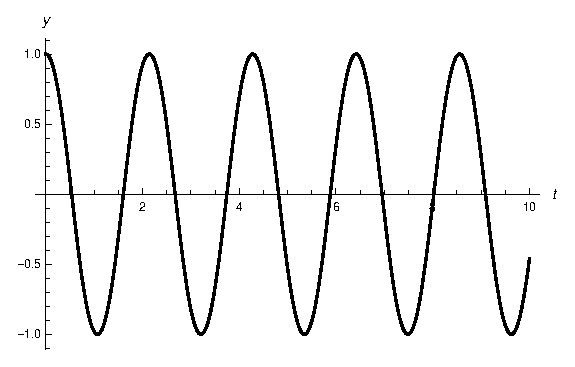
\includegraphics[width=10cm]{figures/ND1.eps}
  \caption{Časová závislost výchylky na čase}
  \label{fig:ND1}
\end{figure}

\begin{figure}[h]
  \centering
  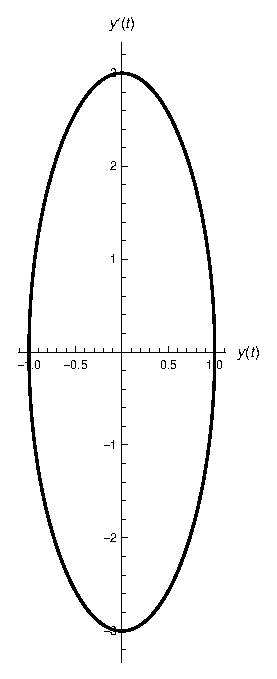
\includegraphics[width=3cm]{figures/ND2.eps}
  \caption{Fázový prostor}
  \label{fig:ND2}
\end{figure}

\begin{figure}[h]
  \centering
  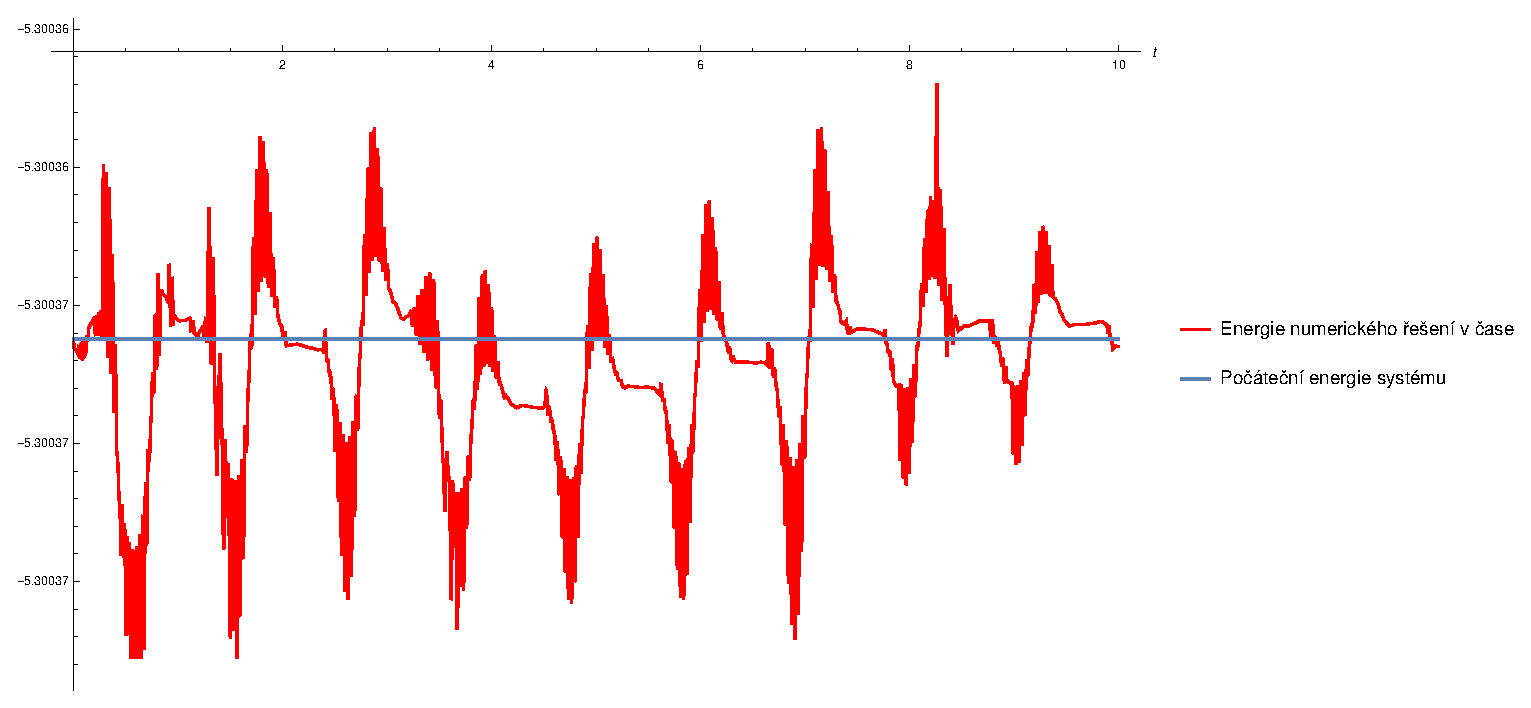
\includegraphics[width=15cm]{figures/ND3.eps}
  \caption{Zachování energie - rovnice $\eqref{ener}$}
  \label{fig:ND3}
\end{figure}

\item[Explicitní Eulerova metoda] 

Tato metoda je nejjednodušší a zároveň, jak si ukážeme, nejméně vhodná pro numerické řešení rovnice $\eqref{rovnice}$. Proto si ji pro ilustraci rozeberme trochu podrobněji. Mějme rovnoměrné (ekvidistantní) dělení $\left\lbrace t_{n} \right\rbrace $ intervalu $(0,10)$:
\begin{equation*}
t_{n} = n h , n \in \mathbb{N_{0}},
\end{equation*}
kde $h$ je velikost kroku. Dále aproximujme $y(t_{n}) \approx y_{n}$. Pak explicitní Eulerova metoda (jednokroková) pro rovnici\footnote{předpokládáme existenci řešení} $y'(t)=f(t,y(t))$ se dá vyjádřit jako\footnote{v našem případě ODR 2. řádu bychom převedli na soustavu ODR 1. řádu}:
\begin{equation*}
y_{n+1} = y_{n} + h f(t_{n},y_{n}).
\end{equation*}
Pro demonstraci získání "špatného" výsledku použijme:
\begin{lstlisting}[language=Mathematica,caption=Eulerova metoda]
NDSolve[{y''[t]+g/l*Sin[y[t]] == 0,y[0] == poc,y'[0] == 0},y, time, Method -> "ExplicitEuler", StartingStepSize -> 0.1,MaxStepSize -> 0.1, MaxSteps -> 100]
\end{lstlisting}

Výsledné numerické řešení naprosto ztrácí periodicitu - obrázek $\eqref{fig:EU1}$ a nezachovává energii $\eqref{fig:EU2}$, $\eqref{fig:EU3}$ - systém energii v čase získává.


\begin{figure}[h]
  \centering
  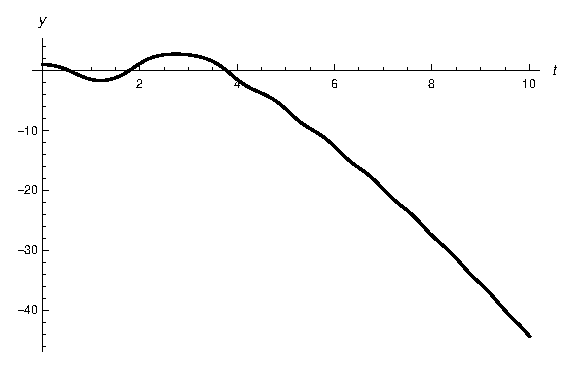
\includegraphics[width=10cm]{figures/EU1.eps}
  \caption{Eulerova metoda - časová závislost výchylky na čase}
  \label{fig:EU1}
\end{figure}

\begin{figure}[h]
  \centering
  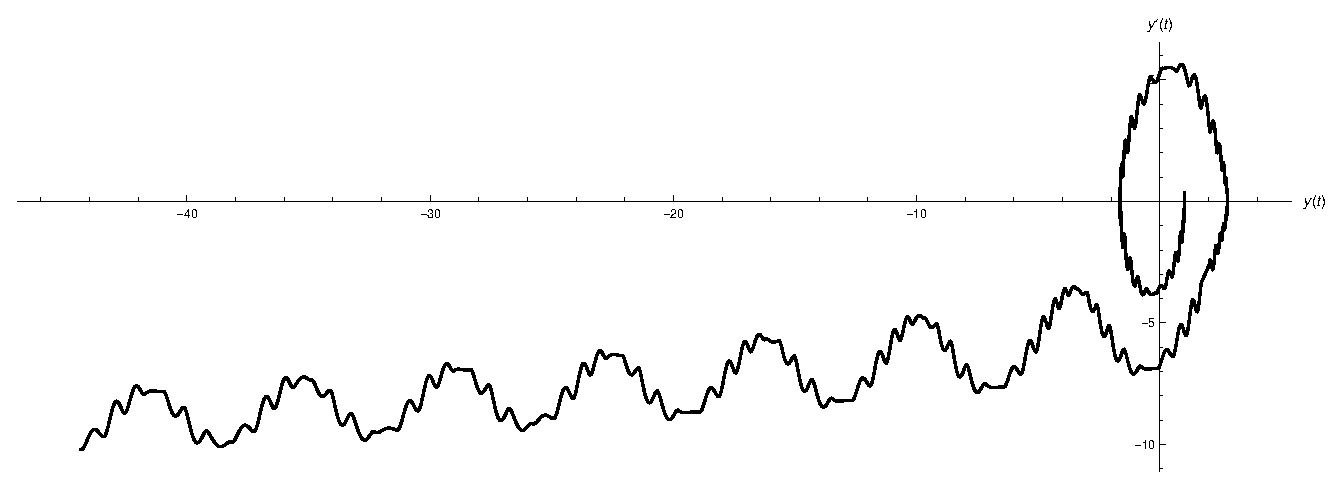
\includegraphics[width=15cm]{figures/EU2.eps}
  \caption{Eulerova metoda - fázový prostor}
  \label{fig:EU2}
\end{figure}

\begin{figure}[h]
  \centering
  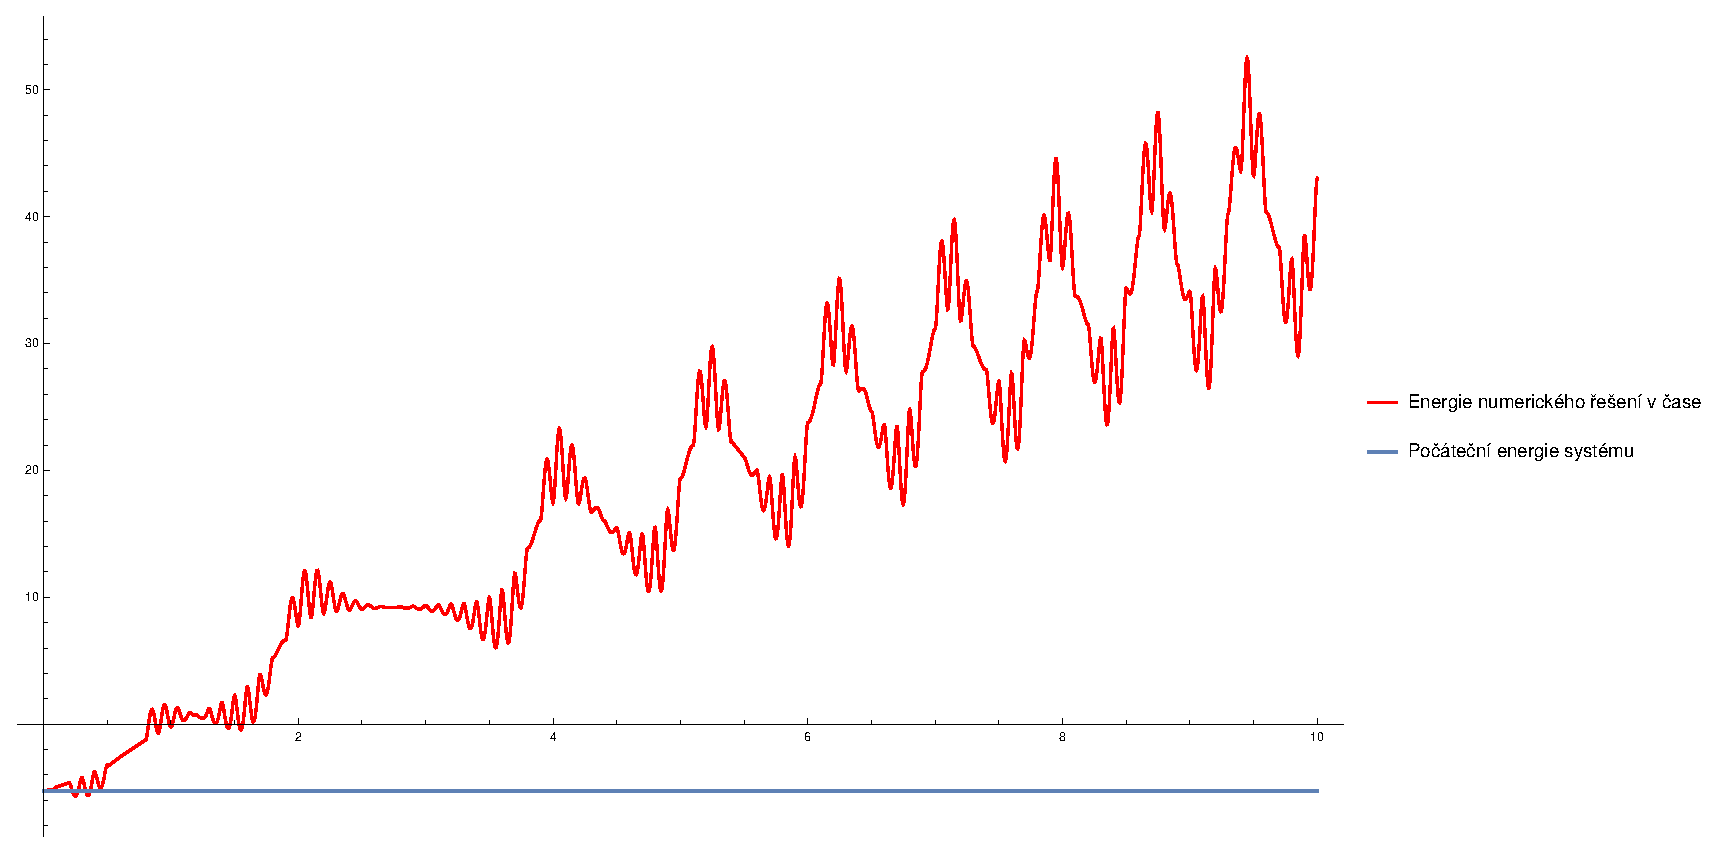
\includegraphics[width=15cm]{figures/EU3.eps}
  \caption{Eulerova metoda - energie}
  \label{fig:EU3}
\end{figure}

\item[Metody snažící se zachovat celkovou energii] 
Nyní použijeme sofistikovanější metody založené na Runge-Kuttových metodách. Pro ilustraci napišme explicitní Runge-Kuttovu metodu 4. řádu (zachováme značení jako výše) pro rovnici~$y'(t)=f(t,y(t))$:
\begin{align*}
K_{1} & = f(t_{n},y_{n}) \\
K_{2} & = f \left(  t_{n}+\frac{h}{2},y_{n}+h\frac{K_{1}}{2} \right)  \\
K_{3} & = f \left(  t_{n}+\frac{h}{2},y_{n}+h\frac{K_{2}}{2} \right)  \\
K_{4} & = f(t_{n}+h,y_{n}+h K_{3}) \\
y_{n+1} & = y_{n}+\frac{1}{6}(K_{1}+2K_{2}+2K_{3}+K_{4})\\
\end{align*}

Konkrétně použijeme metodu \texttt{SymplecticPartitionedRungeKutta}, která ovšem vyžaduje přejít do Hamiltonova formalismu:
\begin{lstlisting}[language=Mathematica,caption=Hamiltonův formalizsmus]
H = p[t]^2/2 - g/l *Cos[q[t]];
eqs = {p'[t] == -D[H, q[t]], q'[t] == D[H, p[t]]};
ics = {p[0] == 0, q[0] == poc};
vars = {q[t], p[t]};
\end{lstlisting}
Máme časově nezávislý hamiltonián - zachovává se v čase (integrál pohybu):
\begin{equation}
H = \frac{p^{2}}{2m} -\frac{g}{l} m \cos(q).
\end{equation}
Implementace metody:
\begin{lstlisting}[language=Mathematica]
NDSolve[{eqs, ics}, vars, time,Method ->{"SymplecticPartitionedRungeKutta","DifferenceOrder" -> 2, "PositionVariables" -> {q[t]}}];
\end{lstlisting}

%\begin{figure}[h]
%  \centering
%  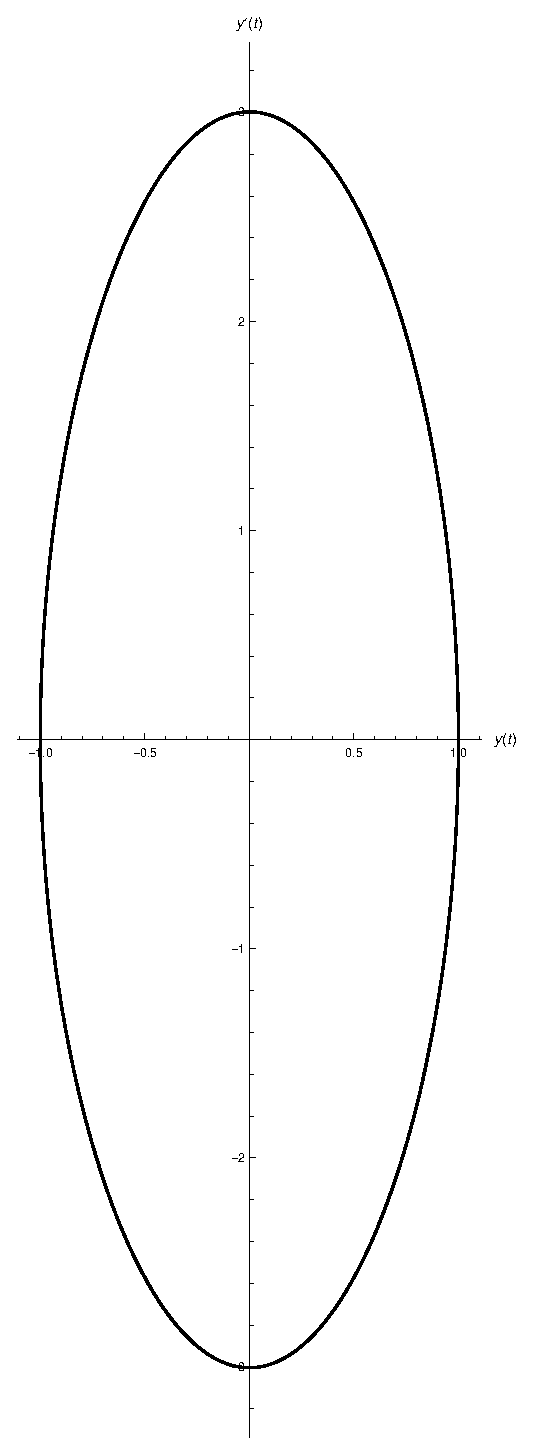
\includegraphics[width=12cm]{figures/SymRK2.eps}
%  \caption{fázový prostor}
%\end{figure}

\begin{figure}[h]
  \centering
  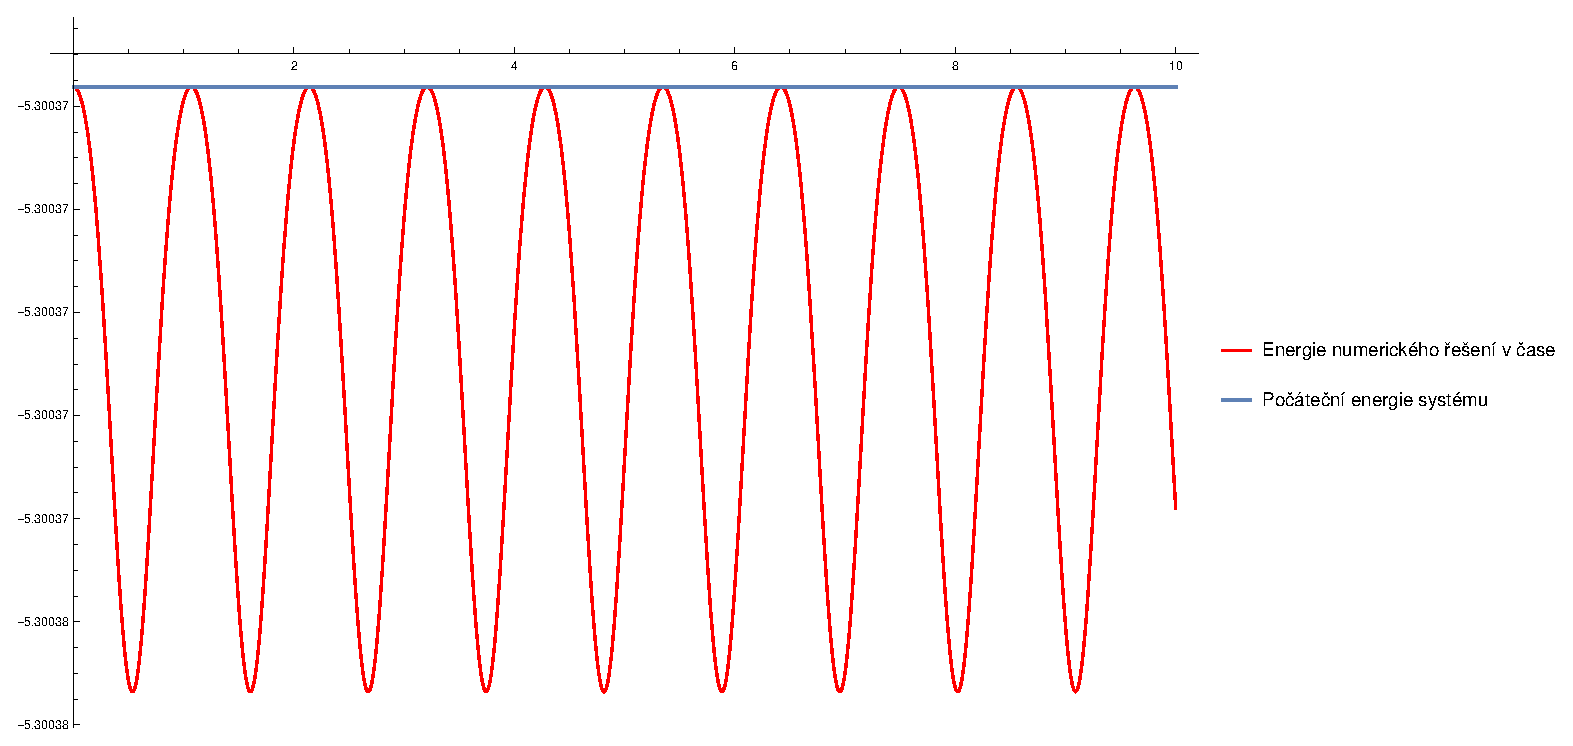
\includegraphics[width=15cm]{figures/SymRK3.eps}
  \caption{Metoda \texttt{SymplecticPartitionedRungeKutta}}
  \label{fig:sprg}
\end{figure}

Řešení dle obrázku $\eqref{fig:sprg}$ též zachovává energii s přesností $10^{-5}$ jako první metoda.

Pro porovnání zkusme ještě jiný přístup pomocí \texttt{Projection}:
\begin{lstlisting}[language=Mathematica]
NDSolve[{y''[t] + g/l *Sin[y[t]] == 0, y[0] == poc,y'[0] == 0}, y, time,  Method -> {"Projection", Method -> "ExplicitRungeKutta", "Invariants" -> -g/l *Cos[poc]}];
\end{lstlisting}
Ale nějakého výrazného zlepšení, již s touto metodou nedocílíme $\eqref{fig:proj3}$.

\begin{figure}[h]
  \centering
  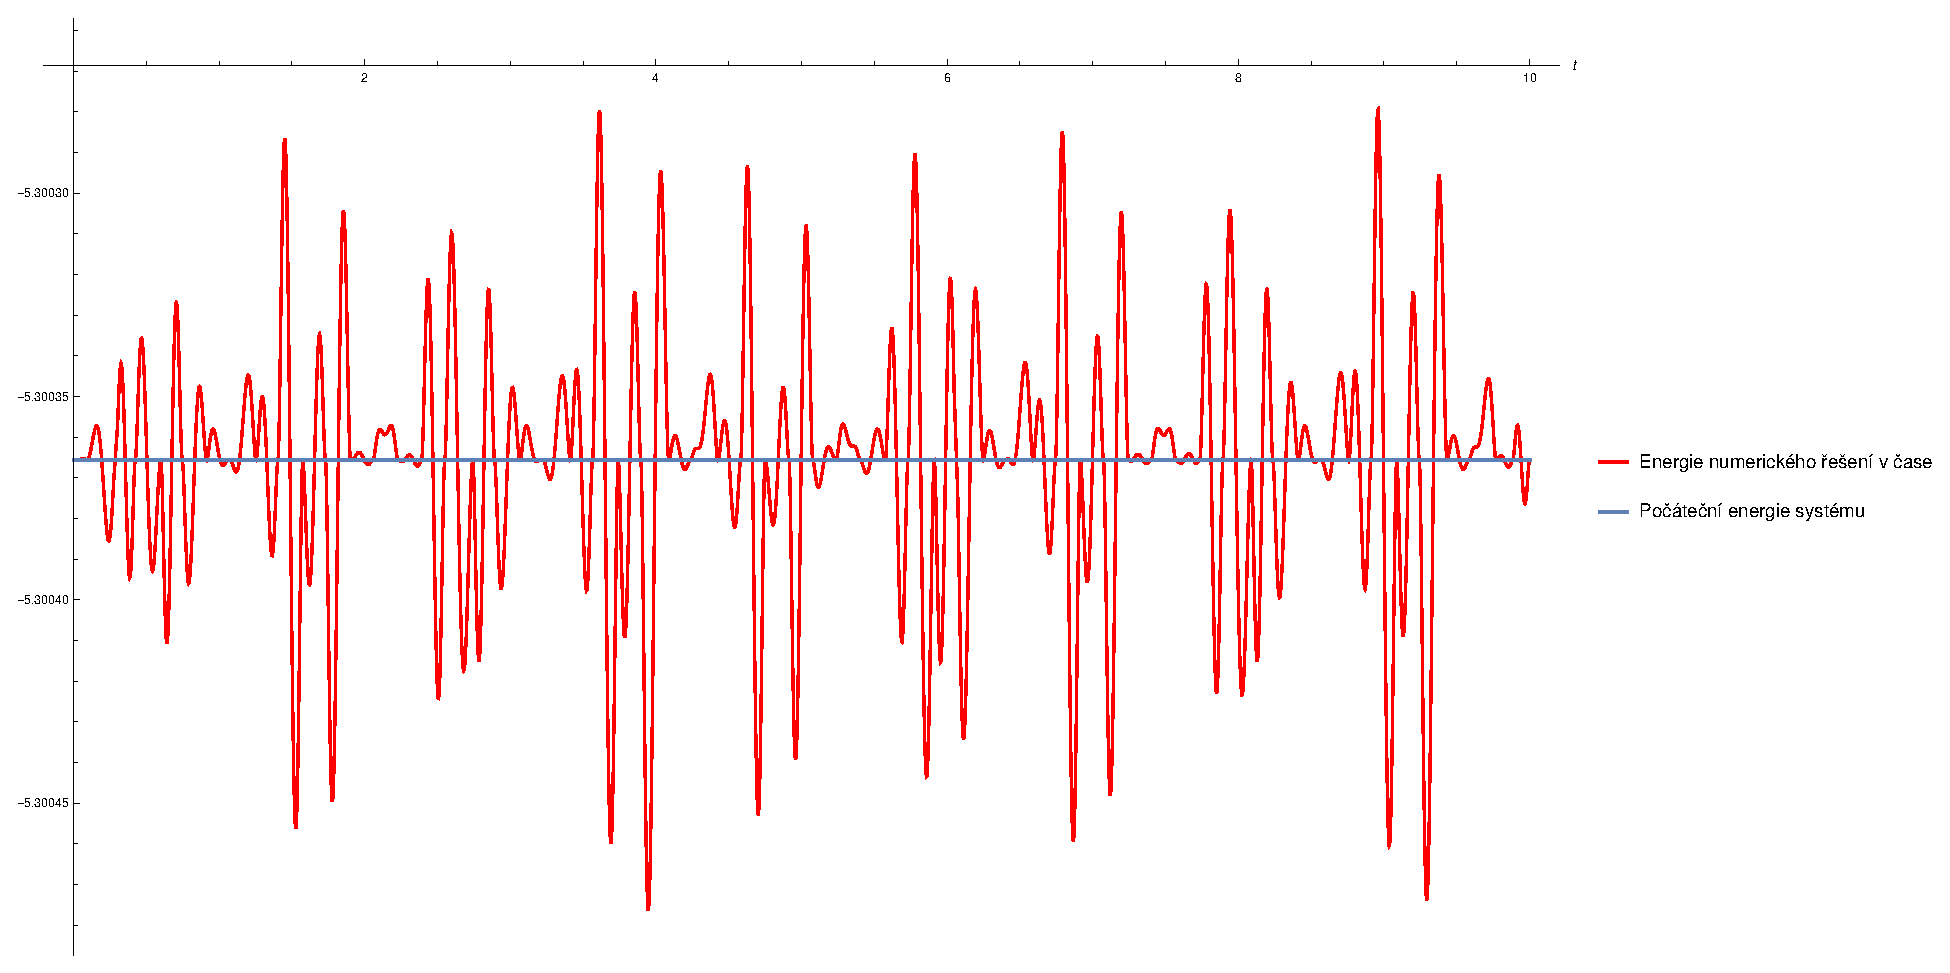
\includegraphics[width=15cm]{figures/Proj3.eps}
  \caption{Projekce}
  \label{fig:proj3}
\end{figure}


\end{description}

\subsection{Perioda kyvadla}
\label{sec:Perioda}

 Lorem ipsum dolor sit amet, consectetuer adipiscing elit. Aliquam erat volutpat. Pellentesque habitant morbi tristique senectus et netus et malesuada fames ac turpis egestas. Fusce aliquam vestibulum ipsum. Integer malesuada. Quis autem vel eum iure reprehenderit qui in ea voluptate velit esse quam nihil molestiae consequatur, vel illum qui dolorem eum fugiat quo voluptas nulla pariatur? Mauris metus. Sed ut perspiciatis unde omnis iste natus error sit voluptatem accusantium doloremque laudantium, totam rem aperiam, eaque ipsa quae ab illo inventore veritatis et quasi architecto beatae vitae dicta sunt explicabo. Ut enim ad minima veniam, quis nostrum exercitationem ullam corporis suscipit laboriosam, nisi ut aliquid ex ea commodi consequatur? Nam sed tellus id magna elementum tincidunt. Nullam eget nisl. Nulla quis diam. Duis condimentum augue id magna semper rutrum.





%%% Local Variables:
%%% mode: latex
%%% TeX-master: "../pendulum"
%%% End:
